\documentclass[]{book}
\usepackage{lmodern}
\usepackage{amssymb,amsmath}
\usepackage{ifxetex,ifluatex}
\usepackage{fixltx2e} % provides \textsubscript
\ifnum 0\ifxetex 1\fi\ifluatex 1\fi=0 % if pdftex
  \usepackage[T1]{fontenc}
  \usepackage[utf8]{inputenc}
\else % if luatex or xelatex
  \ifxetex
    \usepackage{mathspec}
  \else
    \usepackage{fontspec}
  \fi
  \defaultfontfeatures{Ligatures=TeX,Scale=MatchLowercase}
\fi
% use upquote if available, for straight quotes in verbatim environments
\IfFileExists{upquote.sty}{\usepackage{upquote}}{}
% use microtype if available
\IfFileExists{microtype.sty}{%
\usepackage{microtype}
\UseMicrotypeSet[protrusion]{basicmath} % disable protrusion for tt fonts
}{}
\usepackage[margin=1in]{geometry}
\usepackage{hyperref}
\hypersetup{unicode=true,
            pdftitle={MultiPAS User's Guide},
            pdfauthor={Al Fischer},
            pdfborder={0 0 0},
            breaklinks=true}
\urlstyle{same}  % don't use monospace font for urls
\usepackage{graphicx,grffile}
\makeatletter
\def\maxwidth{\ifdim\Gin@nat@width>\linewidth\linewidth\else\Gin@nat@width\fi}
\def\maxheight{\ifdim\Gin@nat@height>\textheight\textheight\else\Gin@nat@height\fi}
\makeatother
% Scale images if necessary, so that they will not overflow the page
% margins by default, and it is still possible to overwrite the defaults
% using explicit options in \includegraphics[width, height, ...]{}
\setkeys{Gin}{width=\maxwidth,height=\maxheight,keepaspectratio}
\IfFileExists{parskip.sty}{%
\usepackage{parskip}
}{% else
\setlength{\parindent}{0pt}
\setlength{\parskip}{6pt plus 2pt minus 1pt}
}
\setlength{\emergencystretch}{3em}  % prevent overfull lines
\providecommand{\tightlist}{%
  \setlength{\itemsep}{0pt}\setlength{\parskip}{0pt}}
\setcounter{secnumdepth}{0}
% Redefines (sub)paragraphs to behave more like sections
\ifx\paragraph\undefined\else
\let\oldparagraph\paragraph
\renewcommand{\paragraph}[1]{\oldparagraph{#1}\mbox{}}
\fi
\ifx\subparagraph\undefined\else
\let\oldsubparagraph\subparagraph
\renewcommand{\subparagraph}[1]{\oldsubparagraph{#1}\mbox{}}
\fi

%%% Use protect on footnotes to avoid problems with footnotes in titles
\let\rmarkdownfootnote\footnote%
\def\footnote{\protect\rmarkdownfootnote}

%%% Change title format to be more compact
\usepackage{titling}

% Create subtitle command for use in maketitle
\newcommand{\subtitle}[1]{
  \posttitle{
    \begin{center}\large#1\end{center}
    }
}

\setlength{\droptitle}{-2em}
  \title{MultiPAS User's Guide}
  \pretitle{\vspace{\droptitle}\centering\huge}
  \posttitle{\par}
  \author{Al Fischer}
  \preauthor{\centering\large\emph}
  \postauthor{\par}
  \date{}
  \predate{}\postdate{}


\begin{document}
\maketitle

\chapter*{}\label{section}
\addcontentsline{toc}{chapter}{}

\textbf{\emph{MultiPAS-III/IV}}

\emph{Multi-laser photoacoustic spectrometers}

\begin{center}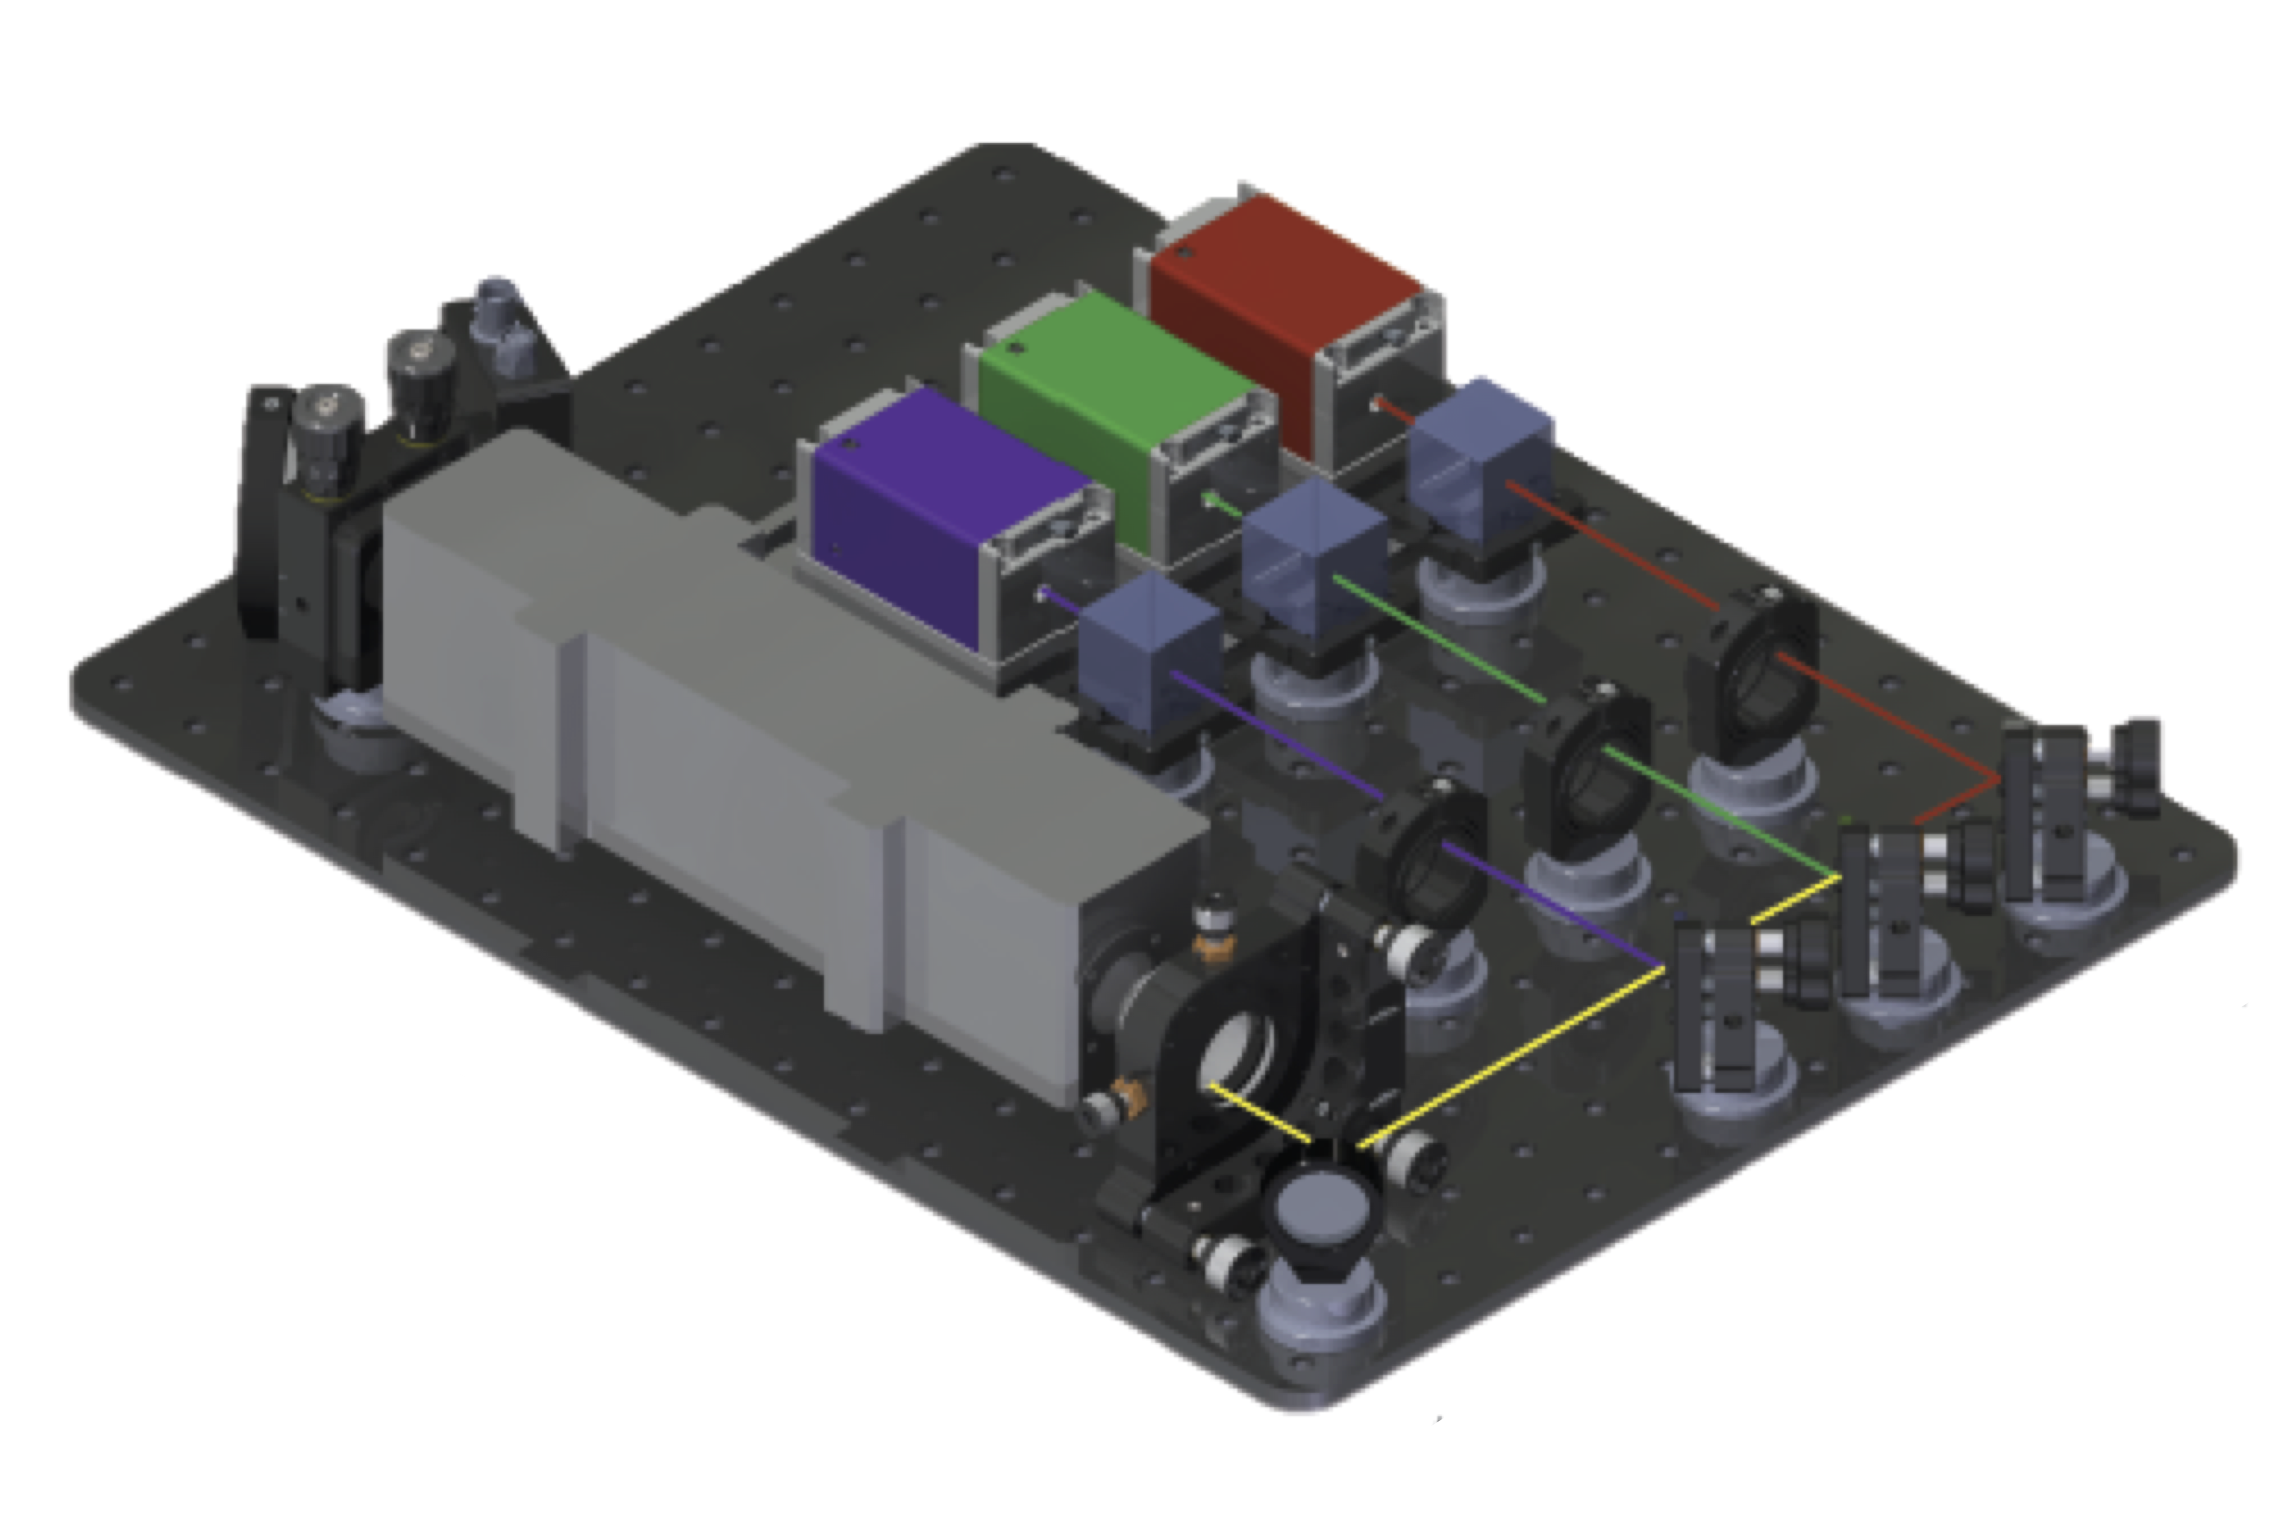
\includegraphics{./images/multiPAS} \end{center}

© 2016 Al Fischer/Smith Lab/University of Georgia

\chapter{Safety Information}\label{safety-information}

Placeholder

\section{Symbol Defintions}\label{symbol-defintions}

\section{Personal Safety Information}\label{personal-safety-information}

\section{Instrument Safety}\label{instrument-safety}

\chapter{Connecting the Instrument}\label{connecting-the-instrument}

Placeholder

\section{Connecting the Control Box}\label{connecting-the-control-box}

\section{Connecting the Microphone}\label{connecting-the-microphone}

\chapter{Quick Start}\label{quick-start}

Placeholder

\section{Installation}\label{installation}

\section{Powering On}\label{powering-on}

\section{Using the Software}\label{using-the-software}

\section{Powering Off}\label{powering-off}

\chapter{Calibration}\label{calibration}

Placeholder

\section{Setup}\label{setup}

\section{Calibration Procedure}\label{calibration-procedure}

\chapter{Data Processing}\label{data-processing}

Placeholder

\section{Processing Data with R}\label{processing-data-with-r}

\subsection{The aeRo Package}\label{the-aero-package}

\subsection{Loading data into R}\label{loading-data-into-r}

\subsection{Exploring MultiPAS Data}\label{exploring-multipas-data}

\subsection{Processing The Data}\label{processing-the-data}

\subsection{Plot data}\label{plot-data}

\chapter{Flow System}\label{flow-system}

Placeholder

\section{Pull Mode}\label{pull-mode}

\section{Push Mode}\label{push-mode}

\chapter{Electrical}\label{electrical}


\includegraphics[width=50px]{./images/warning_highVoltage}

\begin{quote}
\textbf{\emph{Unplug all power before any electrical work on the PAS or
opening the control box!}}
\end{quote}

A genralized diagram of the PAS electrical system is shown below. Some
components, such as photodiodes and the microphone, may require external
power supplies, but the majority of the components are powered directly
via the PAS control box.

\begin{center}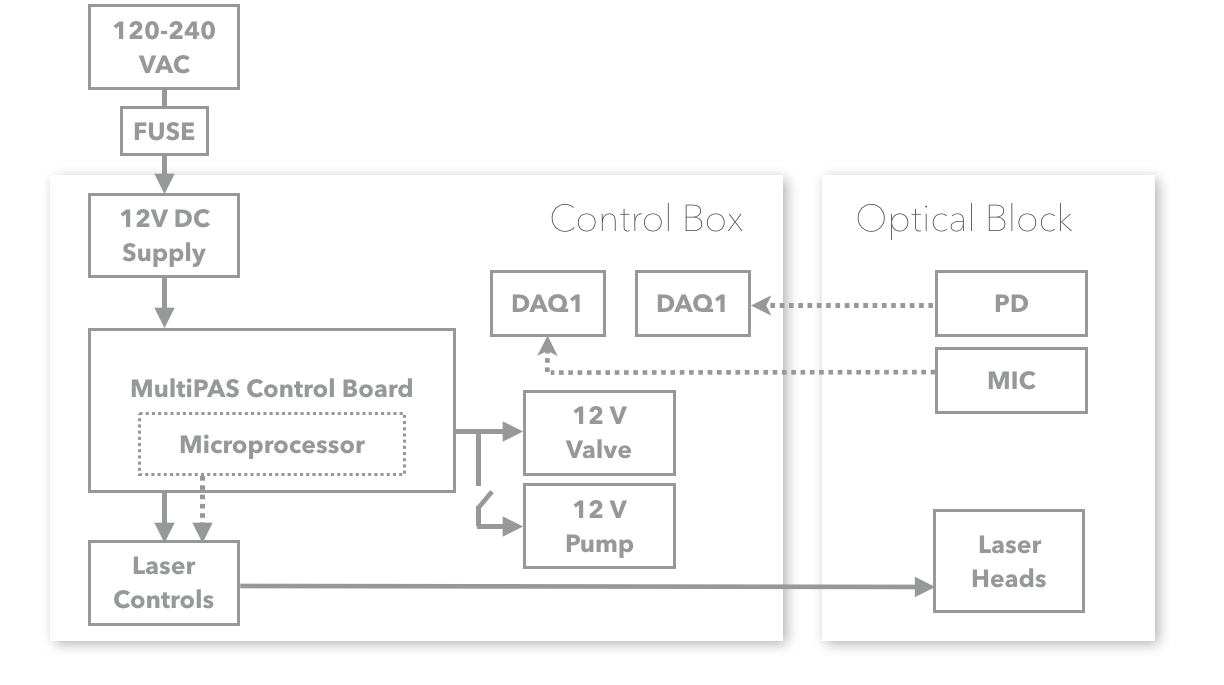
\includegraphics{./images/electricalDiagram} \end{center}

The heart of the PAS electrical system is the Teensy 3.6 (PJRC.com)
microcontroller that resides on the MultiPAS control board. The Teensy
communicates with the software to control the modulation of the lasers
and switch the background valve on and off. The same board distributes
12 V power to the system. The MultiPAS control board may be used with
both 3- and 4-wavelength versions of the PAS. Three-wavelength versions
may have a Teensy 3.2 instead of the 3.6 shown on the schematic; these
are, however, mostly drop-in compatible.

\begin{center}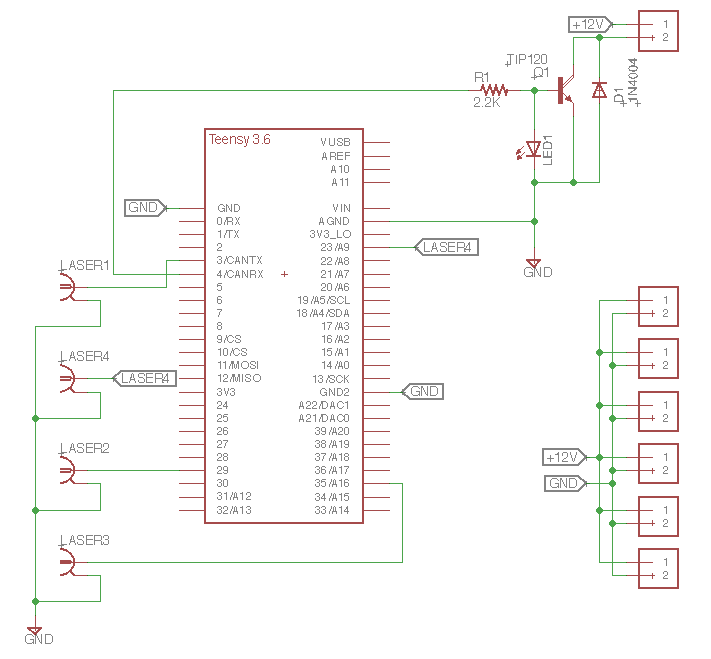
\includegraphics{./images/electricalSchematic} \end{center}

\chapter{Maintainance}\label{maintainance}

Placeholder

\section{HEPA Filter Replacement}\label{hepa-filter-replacement}

\section{Protection Filter
Replacement}\label{protection-filter-replacement}

\section{Cleaning the Orifice}\label{cleaning-the-orifice}

\section{Cleaning the Optics}\label{cleaning-the-optics}

\section{Cleaning the PAS}\label{cleaning-the-pas}

\section{O-ring Replacement}\label{o-ring-replacement}

\section{Fuse Replacement}\label{fuse-replacement}

\section{Realignment}\label{realignment}

\subsection{Multipass Cell}\label{multipass-cell}

\subsection{Beam Steering Optics and
Lasers}\label{beam-steering-optics-and-lasers}

\chapter{Troubleshooting}\label{troubleshooting}

\section{Common Software Errors}\label{common-software-errors}

\begin{enumerate}
\def\labelenumi{\arabic{enumi}.}
\tightlist
\item
  \emph{VISA Read/Write: Device not found.} Either the incorrect COM
  ports have been selected or the USB communication has frozen. In the
  case of the latter, exit LabVIEW completely and reset the PAS by
  turning off the main power switch on the control box \emph{and}
  disconnecting the USB cable. Reconnect and restart.
\item
  \emph{VISA Read/Write: Device is valid but VISA cannot open it.}
  Another program is communicating with one of the PAS's components.
  Close other programs and restart LabVIEW.
\item
  \emph{Valve will not switch and/or frequencies will not change.} USB
  communication broken -- exit LabVIEW completely and reset the PAS by
  turning off the main power switch on the control box \emph{and}
  disconnecting the USB cable. Reconnect and restart.
\item
  \emph{WaveIO Device Not Found.} Known bug with unknown cause. To fix,
  stop the program, increase the PD and mic device ID's (under the
  Utilities tab) by 1 and start the program. Then, stop the program, set
  them back to their original values and start the program again. The
  errors should go away after the final restart.
\item
  \emph{Extremely fast aquisition (x-axis) on PD or mic plots.} See
  \emph{WaveIO Device Not Found}, above.
\end{enumerate}

\section{Common Hardware Errors}\label{common-hardware-errors}

\begin{enumerate}
\def\labelenumi{\arabic{enumi}.}
\tightlist
\item
  \emph{No Signal or Excessive Noise.} Excessive noise or a cancellation
  of signal may occur if:

  \begin{itemize}
  \tightlist
  \item
    \emph{There is an opening on the PAS cell.} Make sure the inlet and
    outlet are attached to the control box, a gas line, or plugged;
    check all fittings on the PAS cell to ensure they are tight.
  \item
    \emph{The pump is not set correctly or the orifice is missing.}
    Lower the pump speed with the trim pot on the pump and check that
    the orifice is in place.
  \item
    \emph{The flow rate is too high.} Lower the flow rate.
  \end{itemize}
\item
  \emph{High Background.} The cell may be dirty. See
  \href{maintainance.html\#cleaning-the-pas}{Cleaning the PAS}.
\item
  \emph{Low Laser Powers.} Low laser power may be observed if:

  \begin{itemize}
  \tightlist
  \item
    \emph{The multipass alignment is bad.}
    \href{maintainance.html\#realignment}{Align} the multipass cell.
  \item
    \emph{The optics are dirty.}
    \href{maintainance.html\#cleaning-the-optics}{Clean the optics.}
  \item
    \emph{The optics are misaligned} Go through the
    \href{maintainance.html\#realignment}{realigment} procedure.
  \end{itemize}
\end{enumerate}


\end{document}
